\Variant{02.03.2026 (1-smena)}
\QQ{1}{$\overline{8962ab}$ körinişdagi son $12$ ga qoldiqsiz bölinsa, $a\cdot b$ ning eng katta qiymatini toping.
\Opts{$72$}{$48$}{$64$}{$54$}}
\QQ{2}{Hisoblang:
\[\frac{45\frac{10}{63}-44\frac{25}{84}}{\left(2\frac13-1\frac19\right):4-\frac34}:\frac{31}{32}\]
\Opts{$2$}{$-2$}{$\dfrac12$}{$-\dfrac12$}}
\QQ{3}{Birinçi sonning $10\%$ iga ikkinçi sonning $\dfrac16$ qismi qöşilgani birinçi sonning yarmidan ikkinçi sonning yarmini ayirganimizga teng. Birinçi sonning ikkinçi songa nisbatini toping.
\Opts{$\dfrac35$}{$\dfrac53$}{$\dfrac56$}{$\dfrac65$}}
\QQ{4}{Öquvçi ikkita kitobni $205\,000$ sömga sotib oldi. Agar birinçi kitob narxi $15\%$ ga kamaytirilsa va ikkinçi kitob narxi $20\%$ ga oşirilsa, kitoblarning yangi narxlari özaro teng böladi. Birinçi kitobning narxi ikkinçi kitob narxidan neça sömga qimmat?
\Opts{$30\,000$}{$35\,000$}{$45\,000$}{$40\,000$}}
\QQ{5}{Hisoblang:
\[\left(-1^2\right)^3+\left(-1^3\right)^4+\ldots+\left(-1^{99}\right)^{100}\]
\Opts{$0$}{$98$}{$50$}{$-1$}}
\QQ{6}{Sonlarni kamayiş tartibida joylaştiring:
\[a=\sqrt8+\sqrt3,\qquad b=\sqrt6+2,\qquad c=2\sqrt3+\sqrt2\]
\Opts{$a>b>c$}{$b>a>c$}{$b>c>a$}{$c>a>b$}}
\QQ{7}{Hisoblang:
\[\sqrt[3]{26+15\sqrt3}+\sqrt[3]{26-15\sqrt3}\]
\Opts{$2$}{$3$}{$4$}{$5$}}
\QQ{8}{Arifmetik progressiyaning istalgan $n$ ta dastlabki hadining örta arifmetigi $2n$ ga teng bölsa, progressiyaning öninçi hadini toping.
\Opts{$38$}{$20$}{$40$}{$36$}}
\QQ{9}{Geometrik progressiyada $b_1+b_2+b_3=70$ va $b_1\cdot b_2\cdot b_3=8000$ bölsa, dastlabki beşta hadi yiğindisini toping.
\Opts{$310$ yoki $77{,}5$}{$310$ yoki $77{,}75$}{$330$ yoki $77{,}25$}{$330$ yoki $77{,}5$}}
\QQ{10}{Ifodani soddalaştiring:
\[\frac{x+2y-\frac{4x^2-y^2}x}{y^3+2xy^2-3x^2y}\]
\Opts{$\dfrac1y$}{$\dfrac xy$}{$\dfrac1x$}{$\dfrac1{xy}$}}
\QQ{11}{Agar $x>0$ bölsa, ifodani soddalaştiring:
\[\frac{\sqrt{\frac12\left(\frac{x^2-2}{2x}\right)^2+1}}{\frac1{2x}\left(x^2+2\right)}\]
\Opts{$2$}{$\dfrac1{\sqrt2}$}{$1$}{$\sqrt2$}}
\QQ{12}{Agar $\sin\alpha=-\dfrac45$ $\left(\dfrac{3\pi}2<\alpha<2\pi\right)$ bölsa, $\cos\alpha$ ni toping.
\Opts{$\dfrac35$}{$-\dfrac35$}{$\dfrac5{13}$}{$-\dfrac5{13}$}}
\QQ{13}{Tenglama $\left[-\dfrac\pi2;\,\pi\right]$ oraliqda neçta yeçimga ega?
\[\sqrt3\sin^2x+\sin^22x=\frac{\sqrt3}2-\frac12-\sqrt3\cos2x\]
\Opts{$1$}{$2$}{$3$}{$5$}}
\QQ{14}{Tengsizlikni neçta butun son qanoatlantiradi?
\[\left(\frac12\right)^{x^2+3x}-\frac{2^{-x}}8>0\]
\Opts{$2$}{$3$}{$4$}{çeksiz köp}}
\QQ{15}{Tengsizlikni neçta butun son qanoatlantiradi?
\[\log_{0{,}5}\log_2\log_{x-1}9>0\]
\Opts{çeksiz köp}{$7$ ta}{$3$ ta}{$5$ ta}}
\QQ{16}{Tenglama neçta haqiqiy ildizga ega?
\[\frac4{(x+6)(x-1)}-\frac5{(x+2)(x+3)}=\frac14\]
\Opts{$1$}{$2$}{$3$}{$4$}}
\QQ{17}{Tenglama neçta haqiqiy ildizga ega?
\[(x-6)^4+(x-8)^4=16\]
\Opts{$1$}{$2$}{$3$}{$4$}}
\QQ{18}{Tengsizlikni neçta butun son qanoatlantiradi?
\[\frac{x^2-1}{x^2+1}+x^2-2x+1\le0\]
\Opts{$0$}{$1$}{$2$}{$3$}}
\QQ{19}{Neçta natural son tengsizlikning yeçimi böla olmaydi?
\[x(x-3)^2>0\]
\Opts{$1$}{$2$}{$3$}{çeksiz köp}}
\QQ{20}{Agar $f(x)=\ln x+\ln3$ va $g(x)=2e^x$ bölsa, $g\bigl(f(3)\bigr)$ ni hisoblang.
\Opts{$8$}{$9$}{$18$}{$36$}}
\QQ{21}{Aniq integralni hisoblang:
\[\int_{-1}^1\frac{x^4}{x^2+1}\,dx\]
\Opts{$\dfrac43-\dfrac\pi2$}{$\dfrac43$}{$0$}{$\dfrac\pi2-\dfrac43$}}
\QQ{22}{$y=\dfrac1{x^2+4}$ funksiya grafigiga ötkazilgan urinma absissa öqiga parallel. Uriniş nuqtasi koordinatalarining yiğindisini toping.
\Opts{$1$}{$\dfrac12$}{$\dfrac34$}{$\dfrac14$}}
\QQ{23}{Aylanaga kvadrat içki çizilgan. Aylana radiusi $\sqrt6$ ga teng bölsa, kvadratning yuzini toping.
\qfig{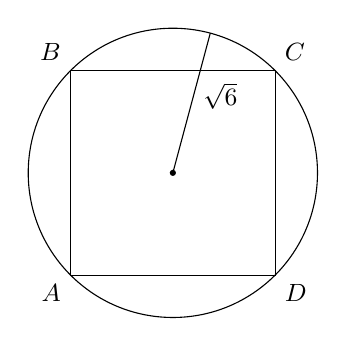
\begin{tikzpicture}[scale=0.75,font=\small]
\draw (0,0) circle (2.449); \draw (-1.732,-1.732) rectangle (1.732,1.732); \draw (0,0)--(75:2.449); \fill (0,0) circle (1.5pt);
\node[below left] at (-1.732,-1.732) {$A$}; \node[above left] at (-1.732,1.732) {$B$}; \node[above right] at (1.732,1.732) {$C$}; \node[below right] at (1.732,-1.732) {$D$};
\node[right] at (0.35,1.3) {$\sqrt6$};
\end{tikzpicture}}
\Opts{$6$}{$12$}{$24$}{$18$}}
\QQ{24}{$|a|>1$, $-1<b\le1$ va $-1\le c<1$ bölsin. $f(x,y,z)=\dfrac{x^2+1}{x^2-1}+\dfrac{2y^2-1}{2y^2+1}+\dfrac{4z^2-1}{4z^2+1}$ funksiyaning $x=\dfrac{\sqrt{a^2-1}}{a-1}$, $y=\sqrt{\dfrac{1-b}{2+2b}}$, $z=\dfrac{\sqrt{1-c^2}}{2(c-1)}$ bölgandagi qiymatini toping.
\Opts{$a+b+c$}{$-1$}{$\dfrac{a+b+c}2$}{$a-b+c$}}
\QQ{25}{Uçburçakning eng katta tomoni $8$ ga, qolgan tomonlari esa $3x-4$ va $2x+1$ ga teng. Agar uçburçakning tomonlari butun sonlardan iborat bölsa, uçburçak perimetrini toping.
\qfig{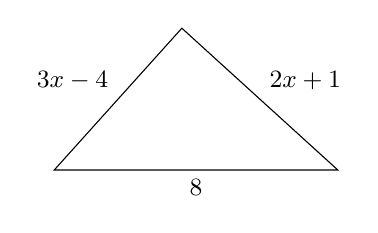
\begin{tikzpicture}[scale=0.45,font=\small]
\draw (0,0)--(8,0)--(3.6,4)--cycle;
\node[above left] at (1.8,2) {$3x-4$}; \node[above right] at (5.8,2) {$2x+1$}; \node[below] at (4,0) {$8$};
\end{tikzpicture}}
\Opts{$16$}{$17$}{$18$}{$20$}}
\QQ{26}{Rasmdagi maʼlumotlar asosida $\alpha$ burçakni toping.
\qfig{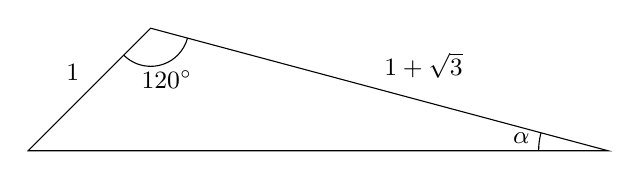
\begin{tikzpicture}[scale=2.2,font=\small]
\coordinate (L) at (0,0); \coordinate (P) at (0.707,0.707); \coordinate (R) at (3.346,0);
\draw (L)--(P)--(R)--cycle;
\draw (P)++(-135:0.22) arc (-135:-15:0.22); \node[below] at (0.8,0.52) {$120^\circ$};
\draw (R)++(180:0.4) arc (180:165:0.4); \node[left] at (2.95,0.07) {$\alpha$};
\node[above left] at (0.35,0.35) {$1$}; \node[above right] at (2.0,0.36) {$1+\sqrt3$};
\end{tikzpicture}}
\Opts{$18^\circ$}{$22{,}5^\circ$}{$15^\circ$}{$36^\circ$}}
\QQ{27}{$ABCD$ teng yonli trapetsiyada $KL$ örta çiziq ötkazilgan. Trapetsiyaning $C$ uçidan $AD$ katta asosiga $CH$ balandlik tuşirildi. $CH$ balandlik $KL$ örta çiziqni $O$ nuqtada kesib ötadi. Agar $KL=48$ va $KO:OL=5:1$ bölsa, $AD$ katta asosni toping.
\qfig{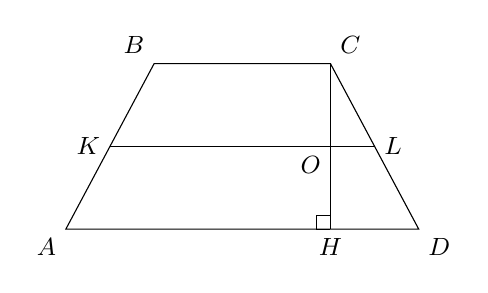
\begin{tikzpicture}[scale=0.07,font=\small]
\coordinate (A) at (0,0); \coordinate (D) at (64,0); \coordinate (B) at (16,30); \coordinate (C) at (48,30); \coordinate (H) at (48,0); \coordinate (K) at (8,15); \coordinate (L) at (56,15); \coordinate (O) at (48,15);
\draw (A)--(B)--(C)--(D)--cycle; \draw (K)--(L); \draw (C)--(H); \draw (48,0)--(45.5,0)--(45.5,2.5)--(48,2.5);
\node[below left] at (A) {$A$}; \node[above left] at (B) {$B$}; \node[above right] at (C) {$C$}; \node[below right] at (D) {$D$}; \node[below] at (H) {$H$};
\node[left] at (K) {$K$}; \node[right] at (L) {$L$}; \node[below left] at (O) {$O$};
\end{tikzpicture}}
\Opts{$54$}{$56$}{$64$}{$72$}}
\QQ{28}{Qavariq $n$ burçakning diagonallari soni $25$ dan kiçik emas va $30$ dan katta emas. $n$ ning qiymatini toping.
\Opts{$9$}{$6$}{$11$}{$7$}}
\QQ{29}{Uçlari $A(1;\,-1;\,-1)$, $B(2;\,2;\,1)$ va $C(3;\,3;\,3)$ nuqtalarda bölgan $ABC$ uçburçak berilgan. $ABC$ uçburçakda $AC$ tomonga $BD$ mediana tuşirilgan. $\cos\angle BDC$ ni toping.
\Opts{$0$}{$\dfrac23$}{$\dfrac13$}{$\dfrac32$}}
\QQ{30}{$\alpha$ tekislikdan taşqarida joylaşgan $A$ nuqtadan uşbu tekislikka $AB$ va $AC$ oğmalar hamda $AH$ perpendikulyar tuşirilgan. Bu yerda $H$ — perpendikulyarning asosi bölib, $B$, $C$ va $H$ nuqtalar $\alpha$ tekislikda yotadi. Agar $AH=4$, $\angle ABH=45^\circ$, $\angle ACH=60^\circ$, $\angle BHC=60^\circ$ bölsa, $AHBC$ piramidaning hajmini toping.
\Opts{$6\dfrac23$}{$5\dfrac23$}{$5\dfrac13$}{$6\dfrac13$}}
\QQ{31}{$A$ töplamga $1$ ta element qöşilgandagi qism töplamlar soni $A$ töplamdan $1$ ta element olingandagi qism töplamlar sonidan $12$ ga köp bölsa, $A$ töplamning qism töplamlari soni neçta?
\Opts{$4$}{$8$}{$16$}{$32$}}
\QQ{32}{$1000$ gaça bölgan natural sonlar içida $11$ ga qoldiqsiz bölinadigan, $2$ ga ham, $3$ ga ham qoldiqsiz bölinmaydigan sonlar neçta?
\Opts{$90$}{$75$}{$45$}{$30$}}
\QQ{33}{\Moslash{Asosining radiusi $6$ cm bölgan silindrga konus içki çizilgan, konusga esa şar içki çizilgan. Konusning asosi va uçi silindr asoslari markazlarida yotadi. Konusning yon sirti $60\pi$ cm$^2$ ga teng.
\par\centering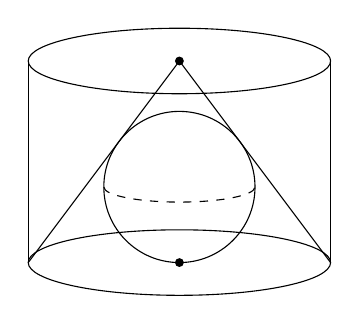
\begin{tikzpicture}[scale=0.32,font=\small]
\draw (0,0) ellipse (6 and 1.3); \draw (0,8) ellipse (6 and 1.3); \draw (-6,0)--(-6,8); \draw (6,0)--(6,8);
\draw (-6,0)--(0,8)--(6,0); \draw (0,3) circle (3); \draw[dashed] (-3,3) arc (180:360:3 and 0.6);
\fill (0,0) circle (5pt); \fill (0,8) circle (5pt);
\end{tikzpicture}}{A) $36\pi$\par B) $96\pi$\par C) $180\pi$\par D) $72\pi$\par E) $192\pi$\par F) $144\pi$}{Silindr va konus töla sirtlarining ayirmasini toping.}{Silindr va konus hajmlari ayirmasini toping.}{Şar hajmini toping.}}
\QQ{36}{Tenglamani yeçing:
\[\sqrt x+2x+2=(x+3)\sqrt[4]x\]
\AB{Tenglama neçta haqiqiy ildizga ega?}{Tenglamaning haqiqiy ildizlari yiğindisini toping.}}
\QQ{37}{Tenglamani yeçing:
\[\sin^3x\,(1+\ctg x)+\cos^3x\,(1+\tg x)=2\sqrt{\sin x\cos x}\]
\AB{Tenglamaning eng kiçik musbat yeçimini toping.}{Tenglama $\left[-\dfrac{5\pi}2;\,\dfrac{5\pi}2\right]$ oraliqda neçta yeçimga ega?}}
\QQ{38}{$f(x)=\dfrac{4x^2}{4x^4+1}$ funksiya berilgan.
\qfig{\begin{tikzpicture}[xscale=1.1,yscale=1.6,font=\small]
\draw[-{Stealth[length=4pt]}] (-3,0)--(3.2,0) node[right] {$x$}; \draw[-{Stealth[length=4pt]}] (0,-0.3)--(0,1.4) node[left] {$y$};
\draw[thick,domain=-2.9:2.9,samples=120] plot (\x,{4*\x*\x/(4*\x*\x*\x*\x+1)});
\node[below left] at (0,0) {$O$};
\end{tikzpicture}}
\AB{Funksiyaning eng katta qiymatini toping.}{Funksiyaning qiymatlar sohasiga neçta butun son tegişli?}}
\QQ{39}{$f(x)=\arctg2^{x-1013}$ funksiya berilgan.
\AB{$f(0)+f(1)+\ldots+f(2026)$ ni toping.}{$f'(1013)$ ni toping.}}
\QQ{40}{Rasmda $f(x)=\dfrac2x$, $y_1=0$, $y_2=2$, $x_1=0$ va $x_2=2$ funksiyalarning grafiklari tasvirlangan.
\qfig{\begin{tikzpicture}[scale=1.1,font=\small]
\fill[qfill] (0,0)--(0,2)--(1,2)--plot[domain=1:2,samples=40] (\x,{2/\x})--(2,0)--cycle;
\draw[-{Stealth[length=4pt]}] (-0.5,0)--(3.3,0) node[right] {$x$}; \draw[-{Stealth[length=4pt]}] (0,-0.5)--(0,3) node[left] {$y$};
\draw[thick,domain=0.7:3,samples=60] plot (\x,{2/\x}) node[above] {$f(x)=\frac2x$};
\draw (-0.2,2)--(2.6,2); \draw (2,-0.3)--(2,2.6);
\node[left] at (0,2) {$y_2=2$}; \node[below right] at (2,0) {$x_2=2$}; \node[below left] at (0,0) {$O$};
\end{tikzpicture}}
\AB{Böyalgan soha yuzini toping.}{Böyalgan sohani $Ox$ öqi atrofida $360^\circ$ ga aylantirişdan hosil bölgan jism hajmini toping ($\pi\approx3$ deb olinsin).}}
\QQ{41}{$ABC$ uçburçakning $AC$ tomonidan $D$ nuqta tanlab olinib, $B$ uçi bilan tutaştirildi. $ABD$ va $BDC$ uçburçaklarga mos ravişda $O_1$ va $O_2$ markazli aylanalar içki çizilgan. Agar $AB=10$, $BC=14$, $AD=10$ va $DC=6$ bölsa,
\qfig{\begin{tikzpicture}[scale=0.4,font=\small]
\coordinate (A) at (0,0); \coordinate (C) at (16,0); \coordinate (D) at (10,0); \coordinate (B) at (5,8.66); \coordinate (O1) at (5,2.887); \coordinate (O2) at (11,1.732);
\fill[qfill] (O1)--(O2)--(D)--cycle;
\draw (A)--(B)--(C)--cycle; \draw (B)--(D); \draw (O1) circle (2.887); \draw (O2) circle (1.732); \draw (O1)--(O2)--(D)--cycle;
\fill (O1) circle (3pt); \fill (O2) circle (3pt);
\node[below left] at (A) {$A$}; \node[above] at (B) {$B$}; \node[below right] at (C) {$C$}; \node[below] at (D) {$D$};
\node[above left] at (O1) {$O_1$}; \node[above right] at (O2) {$O_2$};
\node[left] at (2.5,4.33) {$10$}; \node[above right] at (10.5,4.33) {$14$}; \node[below] at (5,0) {$10$}; \node[below] at (13,0) {$6$};
\end{tikzpicture}}
\AB{$BD$ kesma uzunligini toping.}{$O_1O_2D$ uçburçak yuzini toping.}}
\QQ{42}{$ABCD$ qavariq törtburçakning $AB$, $BC$ va $CD$ tomonlaridan mos ravişda $E$, $F$, $G$ nuqtalar olindi. Bunda $AE:EB=CF:FB=CG:GD=3:4$, $EF=8$, $FG=6$ va $EF\perp FG$ bölsa,
\qfig{\begin{tikzpicture}[scale=0.032,yscale=-1,font=\small]
\coordinate (B) at (380,202); \coordinate (F) at (466,215); \coordinate (C) at (532,222); \coordinate (G) at (518,282); \coordinate (D) at (503,358); \coordinate (A) at (375,347); \coordinate (E) at (378,284);
\draw (A)--(B)--(C)--(D)--cycle; \draw (E)--(F)--(G)--cycle;
\draw ($(F)!0.12!(E)$)--($(F)!0.12!(E)+(F)!0.12!(G)-(F)$)--($(F)!0.12!(G)$);
\node[above left] at (B) {$B$}; \node[above] at (F) {$F$}; \node[above right] at (C) {$C$}; \node[right] at (G) {$G$}; \node[below right] at (D) {$D$}; \node[below left] at (A) {$A$}; \node[left] at (E) {$E$};
\node[above left] at (422,250) {$8$}; \node[above right] at (492,248) {$6$};
\end{tikzpicture}}
\AB{$EFG$ uçburçak yuzini toping.}{$ABCD$ törtburçak yuzini toping.}}
\QQ{43}{Asoslari $3$ va $5$ ga teng bölgan $ABCD$ trapetsiyaga markazlari $O_1$ va $O_2$ bölgan aylanalar mos ravişda içki va taşqi çizilgan. $O_1$ markazli aylana $AB$ va $CD$ yon tomonlarga $E$ va $F$ nuqtalarda urinadi.
\qfig{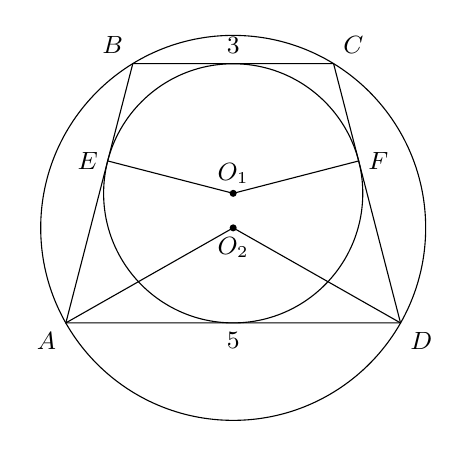
\begin{tikzpicture}[scale=0.85,font=\small]
\coordinate (A) at (-2.5,0); \coordinate (D) at (2.5,0); \coordinate (B) at (-1.5,3.873); \coordinate (C) at (1.5,3.873);
\coordinate (O1) at (0,1.936); \coordinate (O2) at (0,1.42); \coordinate (E) at (-1.875,2.42); \coordinate (F) at (1.875,2.42);
\draw (A)--(B)--(C)--(D)--cycle; \draw (O1) circle (1.936); \draw (O2) circle (2.876);
\draw (E)--(O1)--(F); \draw (A)--(O2)--(D); \fill (O1) circle (1.5pt); \fill (O2) circle (1.5pt);
\node[below left] at (A) {$A$}; \node[above left] at (B) {$B$}; \node[above right] at (C) {$C$}; \node[below right] at (D) {$D$};
\node[left] at (E) {$E$}; \node[right] at (F) {$F$}; \node[above] at (O1) {$O_1$}; \node[below] at (O2) {$O_2$};
\node[above] at (0,3.873) {$3$}; \node[below] at (0,0) {$5$};
\end{tikzpicture}}
\AB{$BCFO_1E$ beşburçak yuzini toping.}{$AEO_1FDO_2$ oltiburçak yuzini toping.}}
\QQ{44}{Barça yon qirralari teng bölgan piramida şarga içki çizilgan. Piramidaning asosi teng yonli trapetsiyadan iborat. Trapetsiyaning yon tomonlari $3$ ga, asoslari esa $5$ va $8$ ga teng. Piramidaning yon qirrasi $\dfrac{14\sqrt3}3$ ga teng bölsa,
\AB{Piramida balandligini toping.}{Şar radiusini toping.}}
\QQ{45}{Rasmda $AB$ qiyalik orqali jism $C$ nuqtaga qarab tortilmoqda. $AB$ qiyalikda $9$ km/soat, $BC$ tekislikda esa $15$ km/soat tezlik bilan tortilmoqda. Bunda $AC=50$ m, $DC=30$ m va $\angle BAD=\alpha$. $A$ nuqtadagi jism eng qisqa vaqt içida $C$ nuqtaga tortib borildi.
\qfig{\begin{tikzpicture}[scale=0.9,font=\small]
\coordinate (A) at (0,0); \coordinate (D) at (4,0); \coordinate (C) at (4,3); \coordinate (B) at (1.5,3);
\fill[qfill] (-0.4,0) rectangle (0,0.4); \draw (-0.4,0) rectangle (0,0.4);
\draw (A)--(D)--(C); \draw[-{Stealth[length=5pt]}] (A)--(B); \draw[-{Stealth[length=5pt]}] (B)--(C); \draw[-{Stealth[length=5pt]}] (A)--(C);
\draw (4,0)--(3.8,0)--(3.8,0.2)--(4,0.2); \draw (A)++(0:0.5) arc (0:63.4:0.5); \node at (0.72,0.36) {$\alpha$};
\node[below] at (A) {$A$}; \node[above] at (B) {$B$}; \node[above right] at (C) {$C$}; \node[below] at (D) {$D$};
\end{tikzpicture}}
\AB{$\cos\alpha$ ni toping.}{Eng kam vaqtni toping (soat).}}
\Javoblar{B B B B A D C A A D B A C B D B B C A C D D B A D C C A B C B D D E A}{\OK{36}{$1$}{$16$}\OK{37}{$\dfrac\pi4$}{$3$}\OK{38}{$1$}{$2$}\OK{39}{$\dfrac{2027\pi}4$}{$\dfrac{\ln2}2$}\OK{40}{$2+2\ln2$}{$18$}\OK{41}{$10$}{$\dfrac{10\sqrt3}3$}\OK{42}{$24$}{$98$}\OK{43}{$\dfrac{3\sqrt{15}}2$}{$\dfrac{19\sqrt{15}}{12}$}\OK{44}{$7$}{$\dfrac{14}3$}\OK{45}{$\dfrac35$}{$\dfrac2{375}$}}
